The choice of cost function is tightly coupled with the choice of output unit. The feedforward network
provides a set of hidden featured defined by $\mathbf{h} = \mathit{f}(\mathbf{x};\mathbf{\theta})$, and
the role of output layer is then to provide some additional transformation from the features to complete 
the task.
\subsection{Linear Units for Gaussian Output Distributions}
Given features $\mathbf{h}$, a layer of linear output units produces a vector 
$\mathbf{\hat{y}} = \mathbf{W}^T\mathbf{h} + \mathbf{b}$. The advantage of a linear unit is that it
never saturates because the slope is always 1. 
They are used to produce the mean of a conditional Gaussian distribution: 
\begin{equation} 
    p(\boldsymbol{y} \mid \boldsymbol{x}) = \mathcal{N}(\boldsymbol{y}; \hat{\boldsymbol{y}}, I). 
\end{equation}
As we saw before, this leads to a \textbf{squared error} for the loss. 
\newline
Furthermore, the network can output two numbers: the mean $\hat{y}$ and a value $v$ for the spread. 
Since the variance must be strictly positive, we set:
\begin{equation}
    s^2 = \zeta(v) = \log(1 + e^v) \quad (\text{always} > 0)
\end{equation}

\begin{figure}[H]
    \centering
    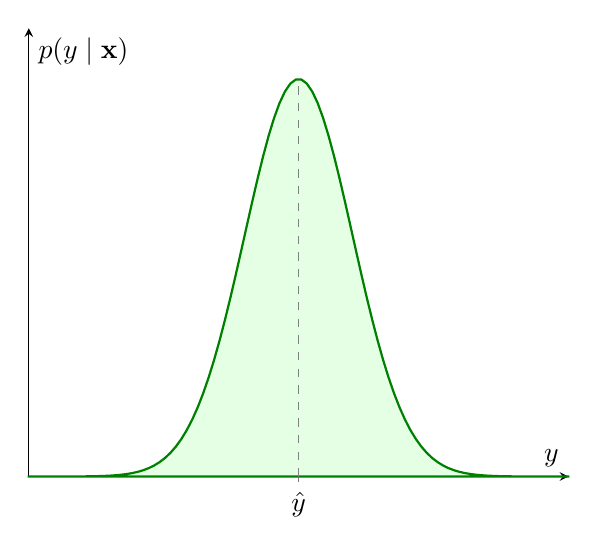
\begin{tikzpicture}
      \begin{axis}[
        xmin=0, xmax=10,
        ymin=0, ymax=0.45,
        axis lines=middle,
        xlabel={$y$},
        ylabel={$p(y \mid \mathbf{x})$},
        xtick={5},
        xticklabels={$\hat{y}$},
        ytick=\empty,
        enlargelimits=false,
        clip=false
      ]
        % Curva gaussiana centrata a x = 5 (rappresenta \hat{y})
        \addplot[domain=0:10, samples=100, color=green!50!black, thick, fill=green!20, fill opacity=0.5] 
          {exp(-((x-5)^2)/(2*1^2)) / (sqrt(2*pi)*1)} \closedcycle;
        
        % Linea tratteggiata dal picco all'asse x
        \draw[dashed, thin, gray] (axis cs:5,0) -- (axis cs:5,0.3989);
      \end{axis}
    \end{tikzpicture}
    \caption{Gaussian Distribution $p(y \mid \mathbf{x})$ centred on $\hat{y}$.}
\end{figure}

\begin{figure}[H]
    \centering
    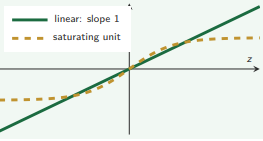
\includegraphics[width=0.3\linewidth]{immagini/linear_unit.png} 
    \caption{Graphical rapresentation of output unit}
    \label{fig:linear_unit}
\end{figure}

\subsection{Sigmoid Units for Bernoulli Output Distributions}
Usefull in classification problems with two classes. A Bernoulli distribution is defined by just a 
single number in the interval [0,1]. The NN needs to predict only $P(y=1 | \mathbf{x})$. The sigmoid
is motivated by constructing an unnormalized probability distribution $\tilde{P}(y)$ which does not sums
to 1.
\begin{align*} 
    \log \tilde{P}(y) &= yz, \\ 
    \tilde{P}(y) &= \exp(yz), \\ 
    P(y) &= \frac{\exp(yz)}{\sum_{y'=0}^{1} \exp(y'z)}, \\ 
    P(y) &= \sigma ((2y - 1)z). 
\end{align*}
The variabile z that defines a distribution over binary variables is called \textbf{logit}.
The loss function for maximum likelihood learning of a Bernoulli parametrized by sigmoid is the 
\textbf{Binary Cross-Entropy}:
\begin{align*}
J(\boldsymbol{\theta}) &= -\log P(y \mid \boldsymbol{x}) \\
&= -\log \sigma ((2y - 1)z) \\
&= \zeta ((1 - 2y)z). \quad \text{(softplus)}
\end{align*}
Using the softplus version, in Fig \ref{fig:BCE} we can see that \textit{saturation} occurs only when 
the model already has the right answer. When \textit{z} has the wrong sign, the argument of the softplus
may be simplified to $|\mathit{z}|$ and so the derivative with respect to \textit{z} asymptotes to $sign(z)$, 
meaning that the gradient won't vanish at all.
If we look at the other loss like  the \textbf{Squared Error}, the loss can saturate anytime 
$\sigma(z)$ saturates (The sigmoid activation function saturates to 0 when z becomes very negative 
and saturates to 1 when z becomes very positive)

\begin{figure}[H]
    \centering
    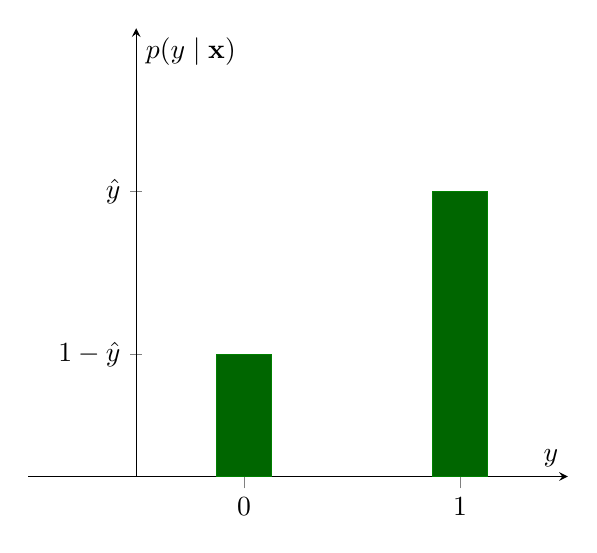
\begin{tikzpicture}
      \begin{axis}[
        xmin=-0.5, xmax=2,
        ymin=0, ymax=1.1,
        axis lines=middle,
        xlabel={$y$},
        ylabel={$p(y \mid \mathbf{x})$},
        xtick={0.5,1.5},
        xticklabels={0, 1},
        ytick={0.3, 0.7},
        yticklabels={$1-\hat{y}$, $\hat{y}$},
        enlargelimits=false,
        ybar,
        bar width=20pt
      ]
        % Barre per Bernoulli (es. probabilità 0.3 per 0 e 0.7 per 1)
        \addplot[fill=green!40!black, draw=green!50!black] coordinates {(0.5,0.3) (1.5,0.7)};
      \end{axis}
    \end{tikzpicture}
    \caption{Bernoulli distribution $p(y \mid \mathbf{x})$ for binary classification.}
\end{figure}
\begin{figure}[H]
    \centering
    \begin{tikzpicture}
    \begin{axis}[
        width = 9cm,
        height = 7cm,
        axis lines = middle,
        xlabel = {$z$},
        ylabel = {$\ell$},
        xlabel style = {right},
        ylabel style = {above},
        xmin = -5.2, xmax = 5.5,
        ymin = -0.5, ymax = 5.5,
        xtick = {-4, -2, 2, 4},
        ytick = {1, 3, 5},
        xticklabel style = {font=\small},
        yticklabel style = {font=\small},
        legend style = {
            at = {(0.5,-0.25)}, 
            anchor = north, 
            legend columns = 2, 
            draw = none, 
            fill = none,
            font = \small
        },
        samples = 200
    ]

    \addplot[domain=-5:5, very thick, green] {exp(-x)};
    \addlegendentry{$y=1$}

    \addplot[domain=-5:5, dashed, very thick, brown] {exp(x)};
    \addlegendentry{$y=0$}

    \end{axis}
    \end{tikzpicture}
    \caption{Loss functions for $y=1$ and $y=0$.}
    \label{fig:BCE}
\end{figure}

\subsection{Softmax Units for Multinoulli Output Distributions}
Useful in classification problems with $k$ classes (categorical outputs). The network needs to produce
a vector $\mathbf{\hat{y}}$ representing the probability distribution over $k$ different classes, 
where each element is in $[0,1]$ and the entire vector sums to 1. The softmax function turns logits 
$\mathbf{z} \in \mathbb{R}^k$ into probabilities:
\begin{align*}
\text{softmax}(\mathbf{z})i &= \frac{e^{z_i}}{\sum{j=1}^k e^{z_j}}, \quad i = 1, \ldots, k
\end{align*}
The loss function for the true class $y$ is the negative log-likelihood:
\begin{align*}
\ell &= -\log \text{softmax}(\mathbf{z})y \ = -z_y + \log \sum{j} e^{z_j}.
\end{align*}
The first term pushes the correct logit up, while the second term pushes all logits down 
(the largest one the most). The gradient of the loss with respect to the logits is:
\begin{align*}
\nabla_{\mathbf{z}}\ell = \text{softmax}(\mathbf{z}) - \mathbf{e}_y
\end{align*}
which represents the prediction minus the one-hot target vector.
\begin{figure}[H]
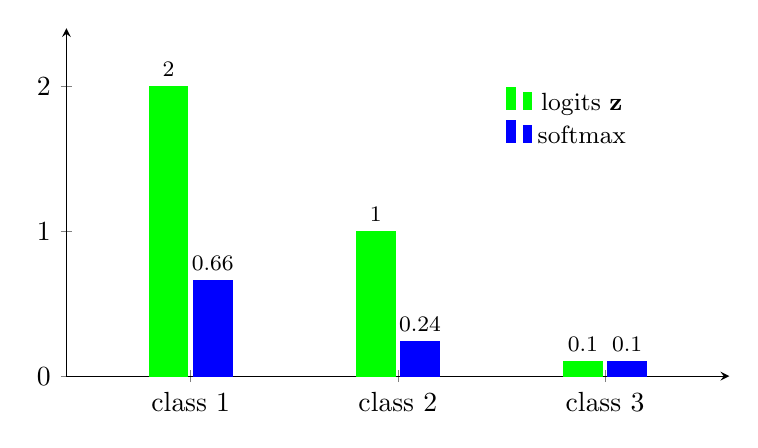
\begin{tikzpicture}
\begin{axis}[
    ybar,
    bar width = 14pt,
    xmin = 0.4, xmax = 3.6, % <-- Qui regoli lo spazio ai lati
    ymin = 0, ymax = 2.4,
    xtick = {1, 2, 3},
    xticklabels = {class 1, class 2, class 3},
    axis lines = left,
    legend style = {
        at = {(0.65, 0.85)},
        anchor = north west,
        draw = none,
        fill = none,
        font = \small
    },
    nodes near coords,
    every node near coord/.append style = {font=\footnotesize, black},
    width = 10cm,
    height = 6cm
]

% Barre per i logit z
\addplot[fill=green, draw=green] coordinates {
    (1, 2)
    (2, 1)
    (3, 0.1)
};
\addlegendentry{logits $\mathbf{z}$}

% Barre per la softmax
\addplot[fill=blue, draw=blue] coordinates {
    (1, 0.66)
    (2, 0.24)
    (3, 0.1)
};
\addlegendentry{softmax}

\end{axis}
\end{tikzpicture}
\end{figure}


\subsection{Mixture Density Networks for Multimodal Targets}
Useful for modeling multimodal targets by representing the conditional probability distribution as a weighted sum of $K$ Gaussian bell curves:
\begin{align*}
p(y \mid \mathbf{x}) = \sum_{c=1}^{K} \pi_c(\mathbf{x}) \mathcal{N}(y; \mu_c(\mathbf{x}), s_c^2(\mathbf{x}))
\end{align*}
The network outputs three groups of parameters for each component $c$:
\begin{itemize}
\item \textbf{Weights $\pi_c(\mathbf{x})$}: constrained via a softmax over $K$ (positive and summing to 1).
\item \textbf{Centres $\mu_c(\mathbf{x})$}: produced by standard linear units.
\item \textbf{Spreads $s_c^2(\mathbf{x})$}: constrained to be positive using softplus ($\zeta$) or exponential functions.
\end{itemize}